\section{Introduction}
\label{sec:intro}
Electromigration (EM) is a physical phenomenon in which metal atoms migrate in response to various driving forces, such as the applied electrical field. In the context of modern very large-scale integration (VLSI) designs, EM remains the dominant reliability failure mechanism for copper-based interconnects, particularly in sub-nanometer technologies. Due to EM, the hydrostatic stress within the metal wire can reach critical levels, leading to resistance variations during migration. This phenomenon results in the formation of voids and hillocks at the cathode and anode, respectively, due to the accumulation and depletion of conducting electrons.
The challenges posed by EM are further exacerbated as technology advances toward nanometer manufacturing processes. In these advanced nodes, the intricate interconnect layouts and the high current densities make EM a critical concern for the long-term reliability and performance of integrated circuits. Addressing EM-related issues becomes increasingly crucial in ensuring the functional integrity and operational lifespan of semiconductor devices in modern electronics.


On-chip power distribution network (PDN), as shown in Fig.~\ref{fig:pgimage}, is a mesh-structured network that provides power to transistors from top metals, directly impacting on-chip performance and reliability. Since PDNs are usually vulnerable to EM-induced failures due to the large and unidirectional current on the PDN. To design robust PDN, designers have to properly size the PDN wires to meet the area and IR drop requirement. This task is changeling as the wires' resistance may change over time due to the EM effect, resulting in IR drops below the threshold voltage  after years of aging effect.
\begin{figure}[htp]
	\centering
	\subfigure[]{
		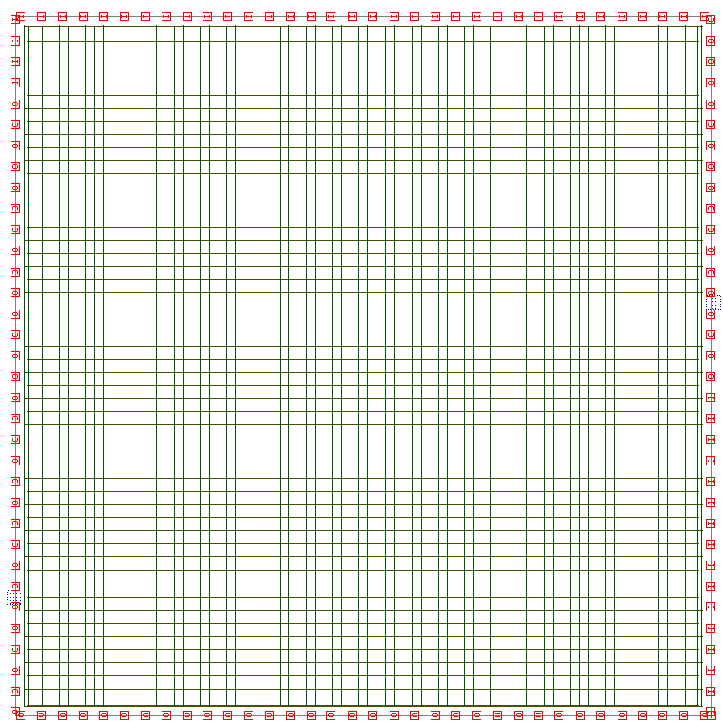
\includegraphics[width=0.4\columnwidth]{./figs/icc2pg.eps}
		\label{fig:icc2pg}}
	\subfigure[]{
		\includegraphics[width=0.48\columnwidth]{./figs/genpg.eps}
		\label{fig:genpg}}
	\caption{(a) Power and ground networks of Cortex-M0 DesignStart; (b) Voltage drop map of the power network of (a).}
	\label{fig:pgimage}
\end{figure}


Numerous past research works have investigated power grid network sizing, utilizing nonlinear or sequence of linear programming (SLP) methods~\cite{ChBr:TCAD'88,DuMa:DAC'89,Tan:DAC'99,Wang:TCAD'05,ZhouSun:TVLSI'19, Sukharev:2019pg,ZhouYu:ASPDAC'20,ZhouJin:ICCAD'20}. Zhou {\it et al.}~\cite{ZhouSun:TVLSI'19,ZhouChen:Integration'21} proposed a power grid sizing approach based on multi-segment EM immortality check criteria. However, this EM immortality-constrained optimization proves too conservative, necessitating all interconnect trees to be immortal. In an effort to address this issue, Moudallal {\it et al.}~\cite{Sukharev:2019pg} proposed a method that directly considers EM-induced IR drops in time-varying power grid networks. This method accounts for post-voiding resistance changes of wires through finite difference analysis of EM-induced stress in multi-segment wires, leading to a nonlinear problem solved via successive linear programming. Nonetheless, this method still incurs high computational costs, as the sensitivities of violating nodes must be computed by solving circuit matrices. More recently, Zhou {\it et al.}~\cite{ZhouJin:ICCAD'20, HanLiu:TCAD'22-23} presented a conjugate gradient-based localized EM-aware IR drop fix for power grid networks, using the generative adversarial networks (GAN)-based deep neural network (DNN) modeling method called {\it GridNet} to compute gradient sensitivities.


Recently, a variational autoencoder (VAE) was proposed for generative applications~\cite{Diederik:arxiv'22}. In contrast to standard autoencoders, the VAE's encoder generates parameters of a predefined distribution in the latent space for each input. Moreover, it introduces additional regularization in the cost function, encouraging the resulting latent distribution to closely approximate the predefined normal distribution, thereby enhancing the reliability of generating new data. VAE has found applications in various fields, including quantum circuit design for drug discovery~\cite{Li:DATE'22}, generative guided analog routing~\cite{Zhu:ICCAD'19}, and analog circuit sizing~\cite{Touloupas:SMACD'22}, underscoring its versatility and potential in different research areas.


Inspired by the generative capabilities of VAE, this paper aims to explore the potential of VAE for efficient prediction of EM-aware IR drop in on-chip power grid networks, to reduce computational costs in power grid design and optimization while ensuring compliance with IR drop and EM lifetime targets. The key contributions of this study are summarized as follows:

\begin{itemlist}

\item  First, we propose a deep neural network model based on VAE structure, called {\it GridVAE}, designed to model full-chip EM-aware IR drop data obtained from numerical EM-aware IR drop analysis tools. By comparing GridVAE with the latest GAN-based model~\cite{ZhouJin:ICCAD'20}, we observe a significant 40\% reduction in Root Mean Square Error (RMSE) based on synthesized power grid benchmark circuits.

\item Second, building upon the new VAE-based EM-aware IR drop models, we leverage its differential nature to fast compute the sensitivity of cost functions to the wire width. This led to an accelerated power grid wire sizing method for ensuring the chip's EM lifetime based on the sequence of linear program optimization framework. Numerical results on a number of synthesized power grid benchmarks from ARM Cortex-M0 processor designs show that the {\it GridVAE} enabled optimization can provide up to over $80$X speedup over the existing analytical matrix solving-based SLP method~\cite{Sukharev:2019pg}.
 
\end{itemlist}

The rest of the paper is organized as follows: Section~\ref{sec:related} reviews the related preliminary works on the EM-induced IR drop analysis and current EM-aware power grid optimization strategy. Section~\ref{sec:strategy} introduces the VAE-based EM-aware IR drop prediction method and the fast full-chip IR drop fixing strategy accelerated by our model. Experiment setup, numerical results, as long as analysis and discussions are summarized in Section~\ref{sec:results}.  Section~\ref{sec:conclusion} concludes the paper.